% FXD: I have commented. Maybe we can do without
% \begin{figure*}
% \centering
% 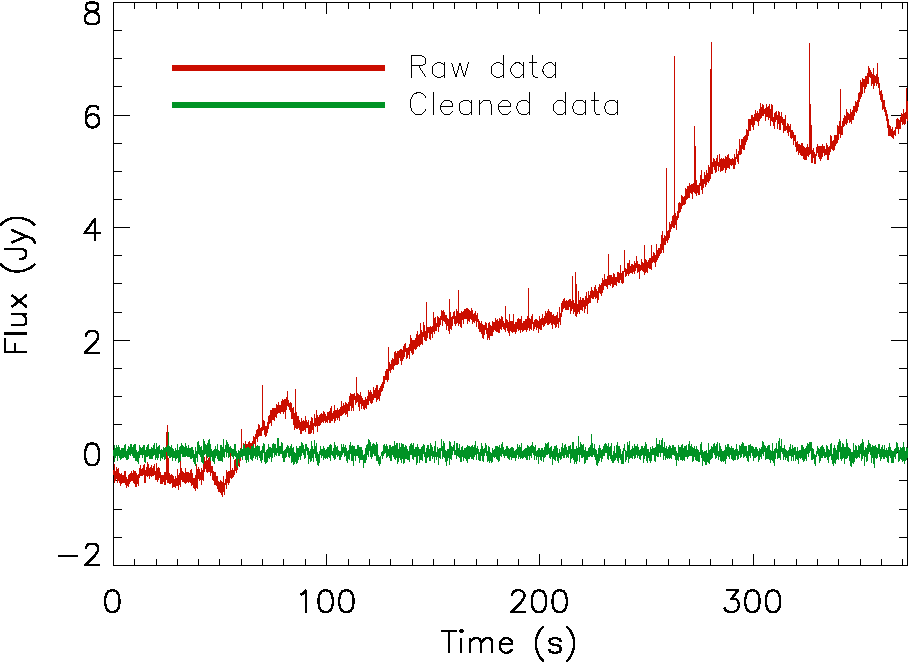
\includegraphics[height=5cm]{figures/TOI_real.ps}
% 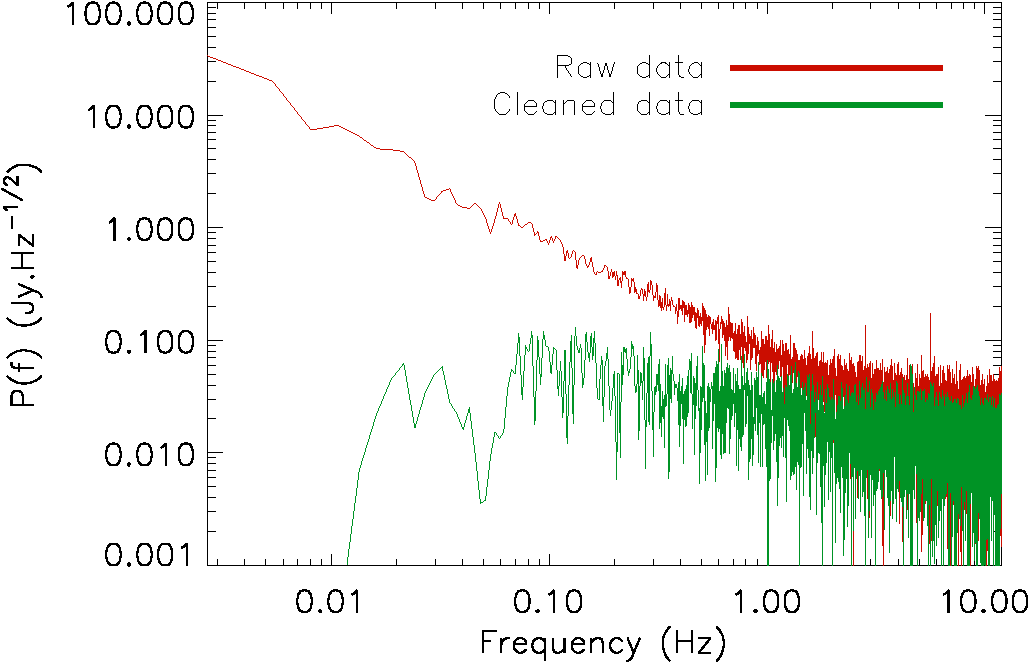
\includegraphics[height=5cm]{figures/PS_real}.ps
% \caption{TOI (left) and power spectra (right) for a given detector. TOI before (red) and after (green) the electronic and atmospheric noise decorrelation. I PUT HERE THE TOI PROCESSING FIGURE FROM ADAM ET AL. PAPER. NEED TO BE CHANGED WITH A SIMILAR FIGURE FOR A PLANET OBSERVATION.}        
% \label{fig:TOI_PS_real}
% \end{figure*}

As discussed in section \ref{REU}, the NIKA data are acquired at 23.842~Hz,
and each pixel is fed a single tone. For each sample and for each KID, the in-phase (I), the
quadrature (Q), and their derivatives (dI and dQ) of the transfer function
of the feed line and the pixel are recovered.
%We recover the in-phase ($I$) and the
%quadrature ($Q$) part of the transfer function of the transmission line and
%KIDs.  
%Thanks to the use of a modulated readout electronics and the
%optimisation procedure (\emph{RFdIdQ}), we can deduce the variation of the
%resonant frequency with an improved accuracy.  
The variation in resonance frequency for each KID in the array is obtained by applying
the optimization procedure, \emph{RFdIdQ}, discussed in Sect.~\ref{sec:rfdidq}.
We developed a dedicated
reduction pipeline to calibrate, filter, and process data onto sky maps.  
The main steps of the processing are:
\begin{itemize}

\item {\bfseries Read raw} : raw data and the main instrumental parameters
including FOV reconstruction and atmospheric
opacity for each observational scan. The data are ordered per kid and
regularly sampled with time. This is called TOI (time ordered information).

\item {\bfseries Flags}: Bad detectors are flagged based on the
  frequency range not being large enough to have a low cross-talk level. 
  Noisy or badly systematic, affected detectors are flagged depending on the statistical 
  properties of their noise (such as Gaussianity, stationarity, noise jumps). 
  Saturated and off-tone KIDs are also flagged out.

 \item {\bfseries Filtering}: Frequency lines produced
  by the vibration of the cryostat pulse tube are flagged and removed with
  dedicated Fourier space filtering.

\item {\bfseries Cosmic rays}: We detect glitches in the raw data. Since
  1.25~mm and 2.14~mm KID arrays are different (in terms of size of the
  pixels and thickness of the substrate), the rate of observed glitches varies
  between them. We observe about six glitches/min in the 2.14~mm array
  and about four for the 1.25~mm array. The observed glitch rate is in
  good agreement with the expected cosmic ray flux at the IRAM telescope,
  which is essentially composed by muons with a rate of about 2 $\mathrm{events / cm^2 /
    min}$ \cite{Ramesh2012}. The time response of the KIDs is hundreds of
  $\mathrm{\mu s}$, which is negligible compared to the NIKA acquisition rate,
  therefore each cosmic ray hit only affects only a single sample. Glitches
  are removed from the TOI by flagging peaks at 5\,$\sigma$ level. Then the
  TOI is linearly interpolated in order not to perturb the decorrelation
  method. Flagged samples are not projected onto the sky.

\item {\bfseries Calibration of the TOI}: The absolute calibration is applied
  to these TOIs and an atmospheric absorption correction performed (see section
  \ref{skydips}).

\item {\bfseries Atmospheric and electronic noise decorrelation}: Depending
  on the scientific target, two basic decorrelation methods have been
  tested:

  1) dual-band decorrelation: spectral decorrelation is performed
  to recover the diffuse thermal SZ effect (see \cite{2013arXiv1310.6237A} for more detail) 
  in clusters of galaxies. We capitalize on the significant difference between the thermal SZ associated signal and
  the two frequency channels. In particular, at 240 GHz the thermal
  SZ emission is negligible to first order, and we can use this channel to obtain a template of the
  atmospheric emission.

  2) single-band decorrelation: a sky noise TOI template is produced by
  averaging all TOIs of a single array. This template is scaled for each
  detector and subtracted from individual TOIs. Variations on this method have
  been tested. They involve masking the point source if bright enough, or
  masking an extended source if detected in a previous iteration of the
  map-making process or filtering the sky noise template.
  In particular, we consider an iterative procedure. A first sky map
  is constructed as discussed above. From this map we construct a mask
  of the source in the TOI. We construct a new TOI sky noise template, avoiding
  samples within the mask. Only a few iterations are needed to converge.
  

So far, the electronic noise has not been dealt with. In general, 
the cross-talk can be due either to resonator coupling or to electronics cross-talk. 
The residual estimated cross-talk in the data is about 2~\%. Decorrelation process 
reduces, or in some case completely removes, the cross-talk. This can limit the sensitivity of
the final sky maps. We are currently investigating how to correct for this by relying on the use of measurements at frequencies that are off-resonance.

%\item {\bfseries Map making} : We project and average the TOI from
%all KIDs of a single array on a pixelized map. Uncertainties on final maps are also computed.

\item {\bfseries map making} : We project and average the TOIs from
all KIDs of a same frequency band on a pixelized map. We do not project flagged data,
and each detector sample is weighted by the inverse variance of the detector
timeline. The latter is estimated far from the source. This weighting scheme
does not average down any residual correlated noise coming from the sky, for
instance. The error bar on flux measurement that we quote is therefore not
computed analytically from these weights but rather from the noise on the map directly.

 Uncertainties on final maps are also computed.


\end{itemize}


%\subsubsection{Glitches}
%Cosmic rays induce glitches in the data. The time response of KIDs due to glitches is negligible compared to the sampling frequency such that they appear as peaks on a single sample in the timelines. We detect about 4 glitches per minute. They are removed from the ${\delta f_0}_k (t)$ timelines by flagging peaks above five times the standard deviation of the considered TOI. The TOIs are interpolated at the glitches location in order not to affect the decorrelation but the final data are not projected onto maps for these points. We can see in figure~\ref{fig:TOI_PS_real} that glitches are present in the raw (calibrated) data (blue) but are removed at the end of the analysis as seen in the red TOI.




